%%%%%%%%%%%%%%%%%%%%%%%%%%%%%%%%%%%%%%%%%%%%%%%%%%%%%%%%%%%%%%%%%%%%%%
% LaTeX Template: Beamer arrows
%
% Source: http://www.texample.net/
% Feel free to distribute this template, but please keep the
% referal to TeXample.net.
% Date: Nov 2006
% 
%%%%%%%%%%%%%%%%%%%%%%%%%%%%%%%%%%%%%%%%%%%%%%%%%%%%%%%%%%%%%%%%%%%%%%
% How to use writeLaTeX: 
%
% You edit the source code here on the left, and the preview on the
% right shows you the result within a few seconds.
%
% Bookmark this page and share the URL with your co-authors. They can
% edit at the same time!
%
% You can upload figures, bibliographies, custom classes and
% styles using the files menu.
%
% If you're new to LaTeX, the wikibook is a great place to start:
% http://en.wikibooks.org/wiki/LaTeX
%
%%%%%%%%%%%%%%%%%%%%%%%%%%%%%%%%%%%%%%%%%%%%%%%%%%%%%%%%%%%%%%%%%%%%%%

\documentclass{beamer} %
\usetheme{Darmstadt}
\usepackage[latin1]{inputenc}
\usefonttheme{professionalfonts}
\usepackage{times}
\usepackage{color}
\usepackage{tikz}
\usepackage{amsmath}
\usepackage{verbatim}
\usepackage[absolute,overlay]{textpos}
\usepackage{graphicx}
\usetikzlibrary{arrows,shapes}
\usepackage{multimedia}


\author{Simon Sternsdorf}
\title{Artistic style transfer for videos}




\begin{document}

\setbeamercolor{item projected}{fg=white, bg=red}
\setbeamerfont{caption}{size=\scriptsize}



% For every picture that defines or uses external nodes, you'll have to
% apply the 'remember picture' style. To avoid some typing, we'll apply
% the style to all pictures.
\tikzstyle{every picture}+=[remember picture]

% By default all math in TikZ nodes are set in inline mode. Change this to
% displaystyle so that we don't get small fractions.
\everymath{\displaystyle}
\begin{frame}
\titlepage
\end{frame}



\section{Introduction}
\begin{frame}
\frametitle{Introduction}


\begin{textblock}{1}(6,3)
	\begin{figure}
	
\includegraphics[scale=0.2]{figures/Prisma}

	\end{figure}
	
 \end{textblock}


\begin{textblock}{5}(4,6)
	\begin{figure}
	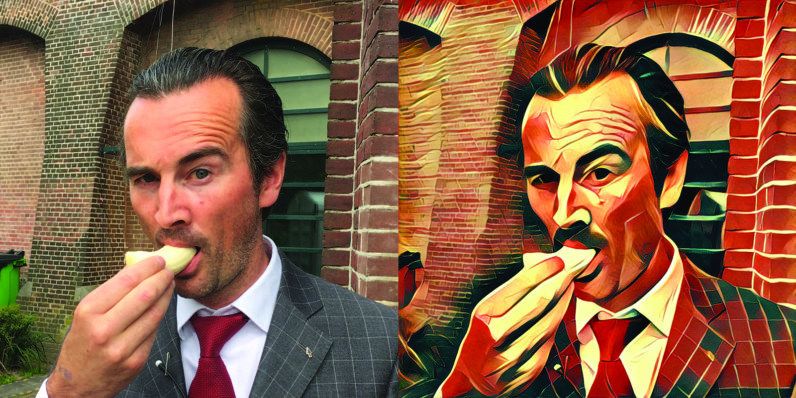
\includegraphics[scale=1]{figures/prisma2}
	\caption{Prisma, the App for AI Powered Art Styles}
	\end{figure}
 \end{textblock} 

\end{frame}



\begin{frame}
\frametitle{Introduction}
\begin{textblock}{1}(1.5,3)
	\begin{figure}
	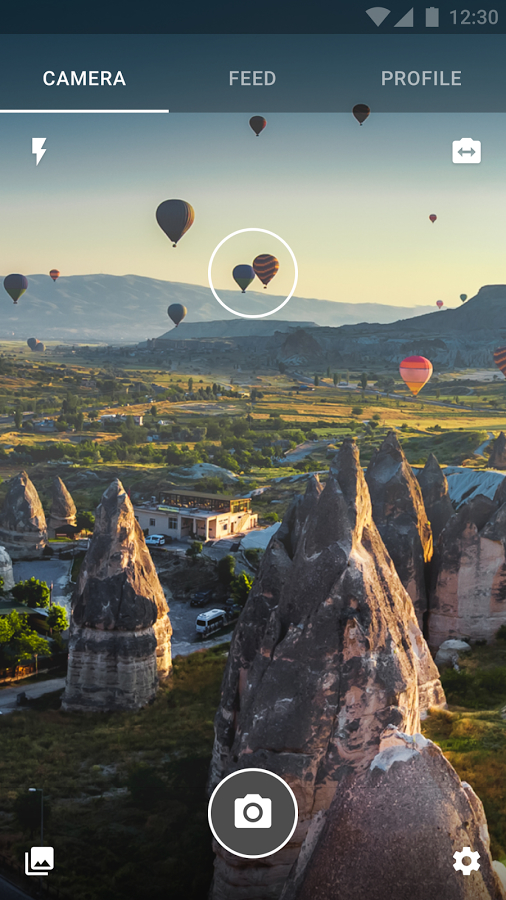
\includegraphics[scale=0.2]{figures/prismaApp2}
	
	\end{figure}
 \end{textblock}
 \begin{textblock}{1}(6.5,8.5)
	$$\longrightarrow$$
 \end{textblock}
\begin{textblock}{1}(8,3)
	\begin{figure}
	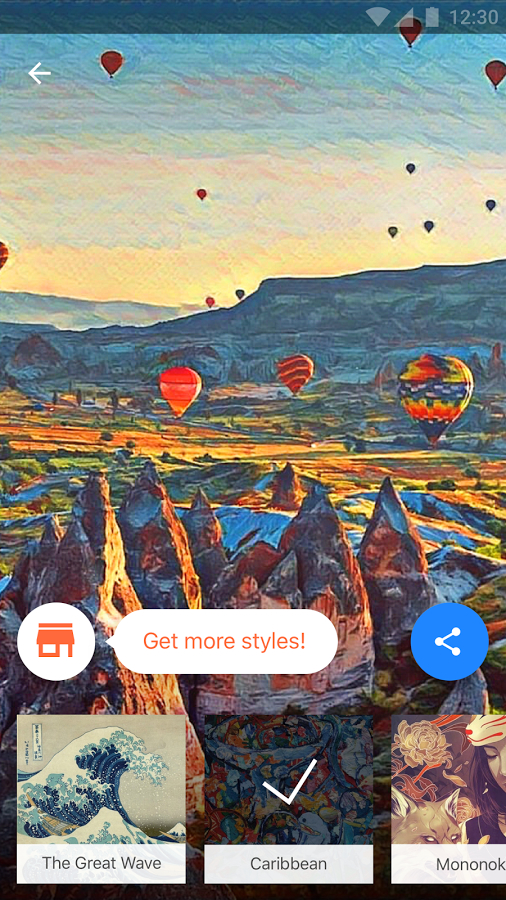
\includegraphics[scale=0.2]{figures/prismaApp1}
	
	\end{figure}
 \end{textblock}

\end{frame}

\begin{frame}
\frametitle{Outline}
\tableofcontents
\end{frame}


\AtBeginSection[]
{
\begin{frame}
\frametitle{Outline}
\tableofcontents[currentsection]
\end{frame}
}






\section{Picture recognition}

\subsection{Biological vision for Neural Networks}
\begin{frame}
\frametitle{Biological vision for Neural Networks}

\textbf{We use Convolutional Neural Networks}
\newline
\pause
\begin{itemize}

	\setlength\itemsep{1em}
	\item Many layers of processing units
	\pause	
	\item Each unit applies image filters
	\pause
	\item Output: Feature map
\end{itemize}



\end{frame}

\begin{frame}
\frametitle{Biological vision for Neural Networks}
\begin{textblock}{5}(1,3)
	\begin{figure}
	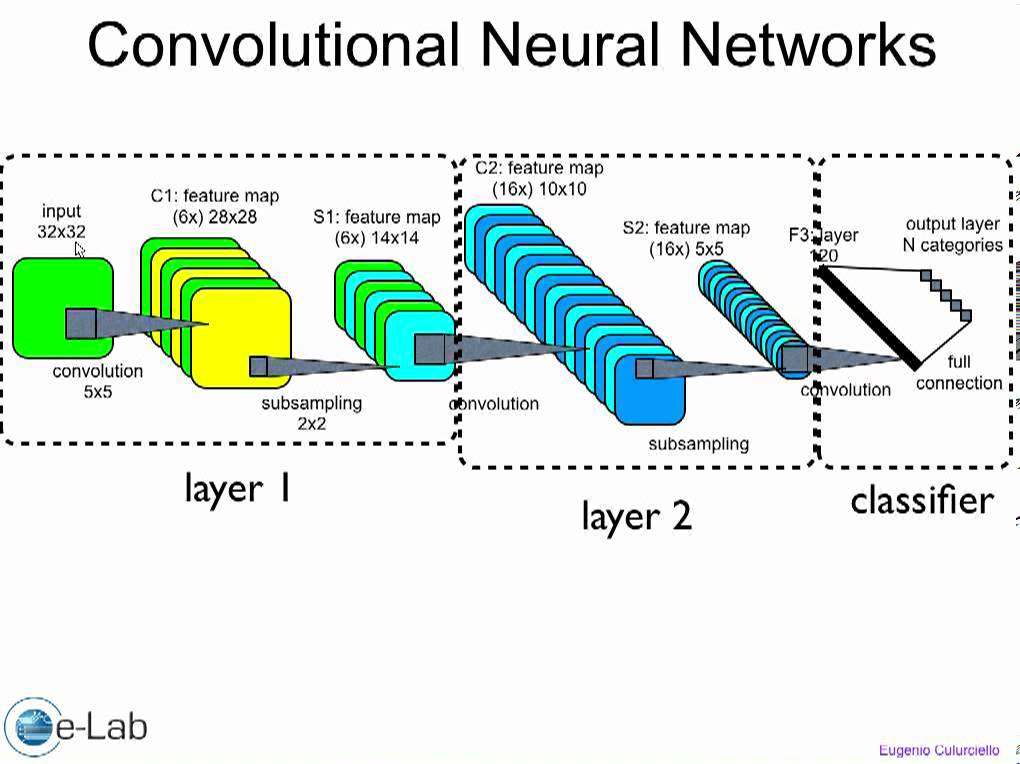
\includegraphics[scale=0.3]{figures/convolution.jpg}
	\caption{Work of a CNN}
	\end{figure}
 \end{textblock} 

\end{frame}

\begin{frame}

\frametitle{Biological vision for Neural Networks}
\begin{textblock}{5}(1,5)
	\begin{figure}
	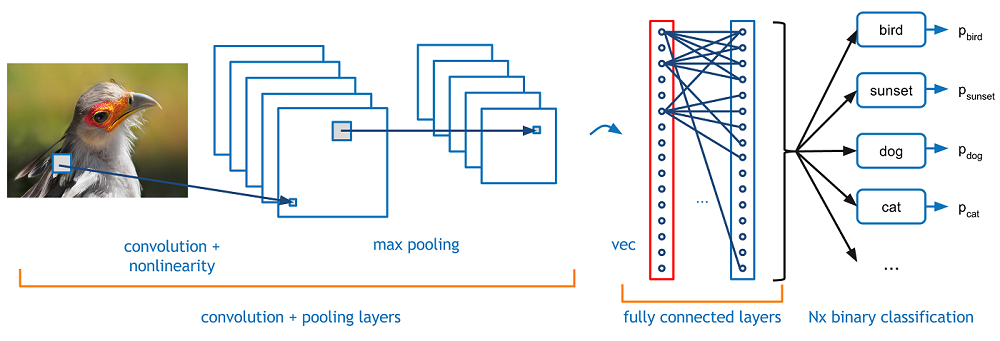
\includegraphics[scale=0.65]{figures/Conv.png}
	\caption{Work of a CNN}
	\end{figure}
 \end{textblock} 


\end{frame}


\subsection{Content and Style}
\begin{frame}
\frametitle{Content and Style}

\begin{textblock}{4}(2,3)
	\begin{figure}
	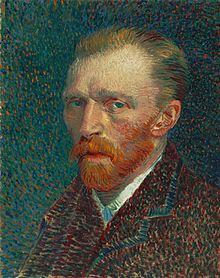
\includegraphics[scale=0.8]{figures/goth}
	\caption{Van Gogh self-portrait }
	
	\end{figure}
	
 \end{textblock} 

\begin{textblock}{6}(8.5,6)
	Difference between content and style?
 \end{textblock} 


\end{frame}

\begin{frame}

\begin{figure}[h]
\centering
{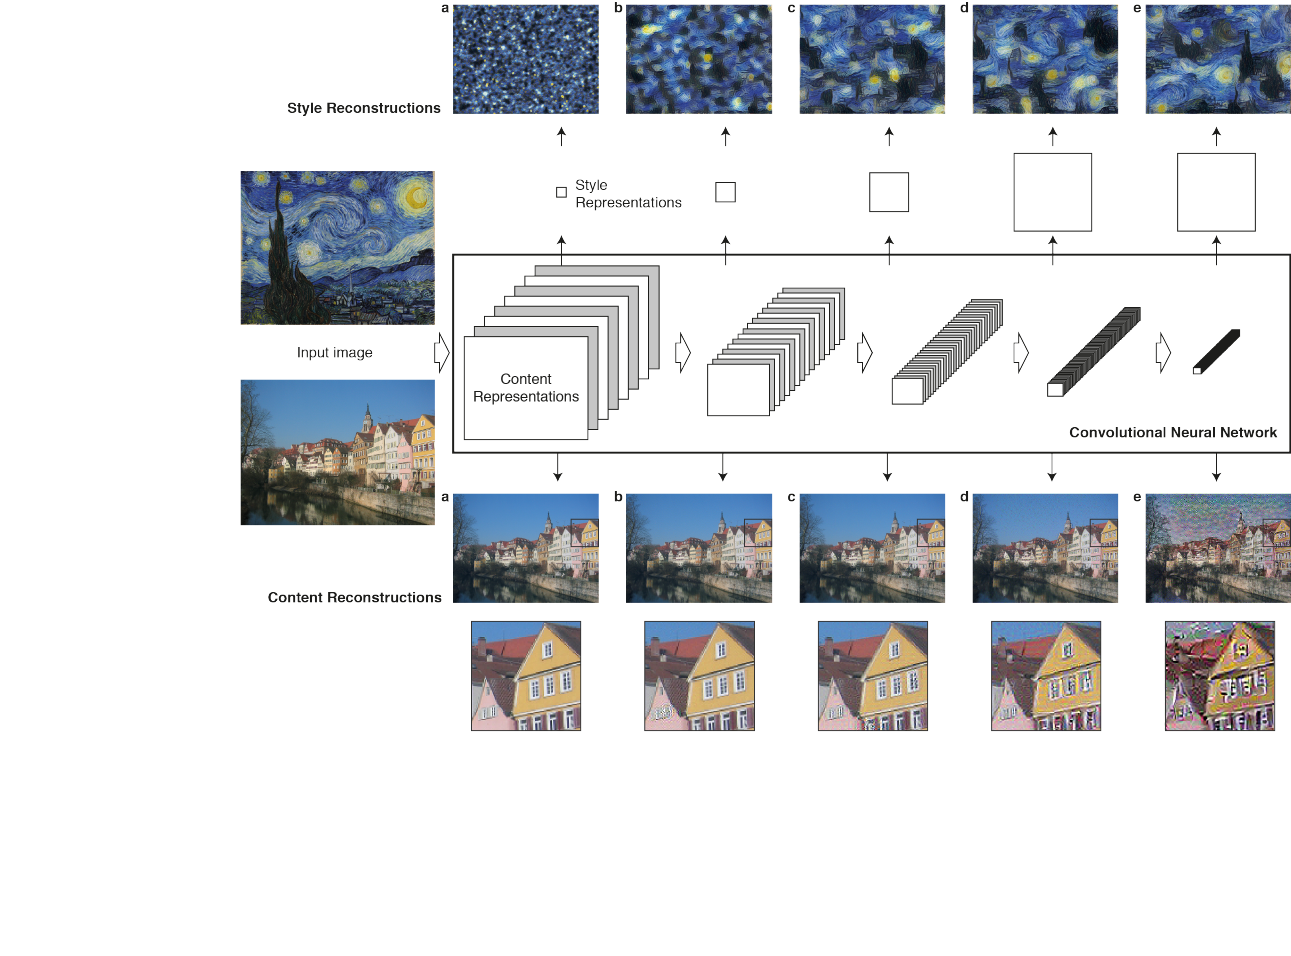
\includegraphics[width=1\columnwidth]{figures/network_model}} \quad


\end{figure}
\begin{textblock}{10}(3,14)
	\textcolor{blue}{Figure}: Model for the network \cite{Paper1}
 \end{textblock} 


\end{frame}

\begin{frame}
\frametitle{Content and Style}
Result:
\begin{itemize}
\item  Representations of content and style in CNNs are separable
\pause
\item Both representations can be changed independently.
\pause
\item $\longrightarrow$ Mix style and content of two source images 
\end{itemize}

\end{frame}

\begin{frame}

\begin{textblock}{5}(3,1)
	\begin{figure}
	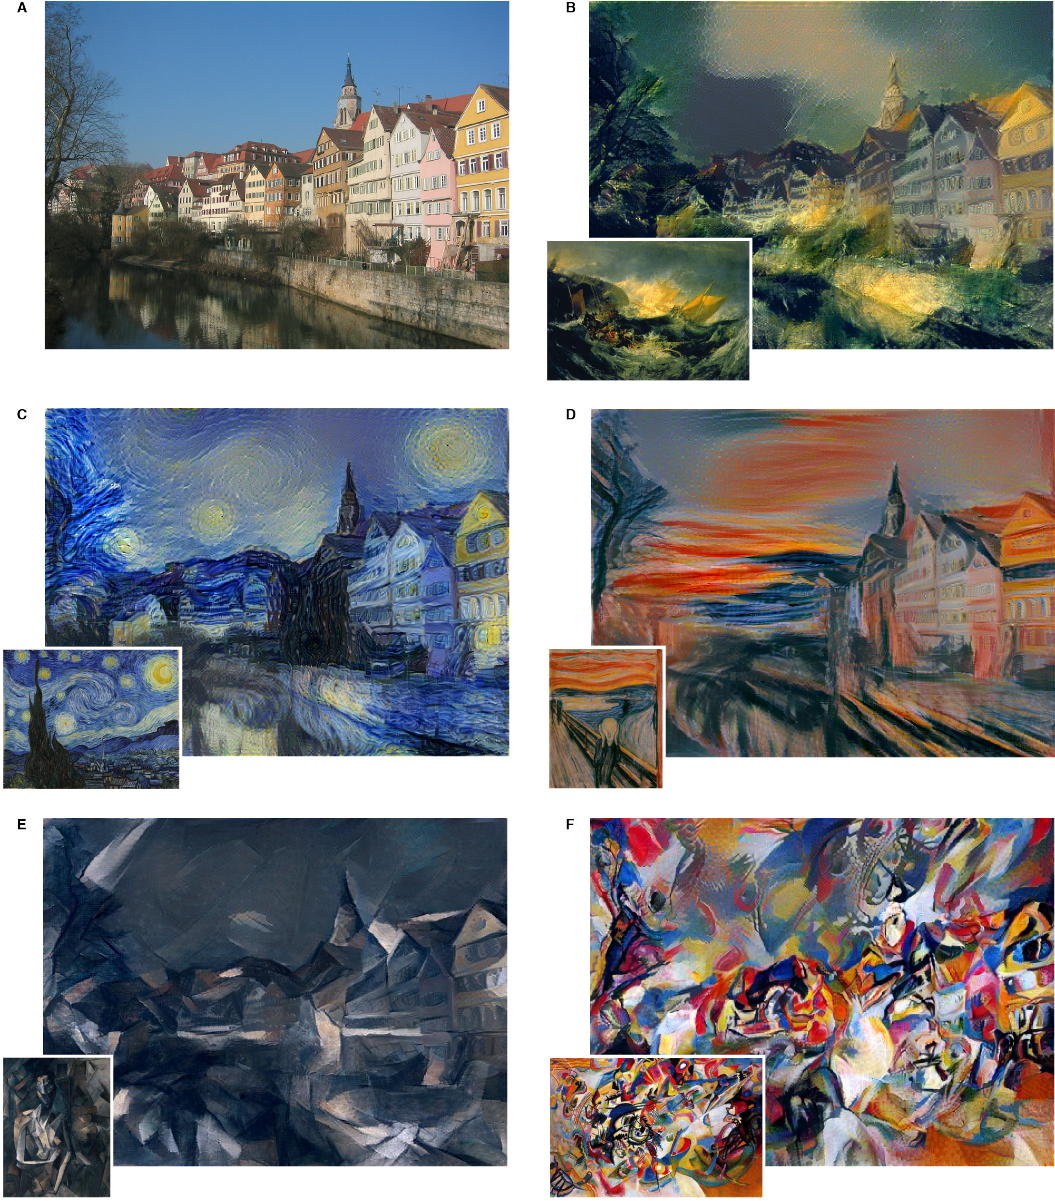
\includegraphics[scale=0.4]{figures/examples.png}
	\caption{Examples}
	\end{figure}
 \end{textblock} 

\end{frame}



\subsection{Encoding of one image}

\begin{frame}
\frametitle{Content reconstruction}
Notation:
\begin{itemize}
\item $\overrightarrow{p} = $ Original Picture, $\overrightarrow{x} =$ initial random image
\item $P^l $ and $F^l$ feature representation in layer $l$
\end{itemize}
$\newline$
$\newline$
Content reconstruction: Encode $\overrightarrow{x}$ until it generates the same response in some layers of the CNN as $\overrightarrow{p}$

\end{frame}

\begin{frame}
\frametitle{Content reconstruction}
Notation:
\begin{itemize}
\item $\overrightarrow{p} = $ Original Picture, $\overrightarrow{x} =$ initial random image
\item $P^l $ and $F^l$ feature representation in layer l
\end{itemize}
$\newline$
\begin{itemize}
\item Set $\overrightarrow{x}$ to a white noise image
\pause
\item Perform gradient descent on the image
\pause
\item $\longrightarrow$ find $\overrightarrow{x}$ that matches feature responses of $\overrightarrow{p}$
\end{itemize}

\end{frame}



\begin{frame}

\begin{itemize}
\frametitle{Style reconstruction}
\item For style reconstruction we basically do the same
\item Perform gradient descent on the image 
\item find $\overrightarrow{x}$ that matches style representation of original image
\end{itemize}
 
\end{frame}

\begin{frame}
\frametitle{Content and style}
In total: When $\overrightarrow{p}$ is the photograph and $\overrightarrow{a}$ is the artwork, we try to minimise the loss function: 
$\newline$
$$\mathcal{L}_{total}(\overrightarrow{p},\overrightarrow{a},\overrightarrow{x}) = \alpha \mathcal{L}_{content}(\overrightarrow{p},\overrightarrow{x}) + \beta \mathcal{L}_{style}(\overrightarrow{a},\overrightarrow{x}) $$

\end{frame}

\begin{frame}

\begin{textblock}{5}(2,1)
	\begin{figure}
	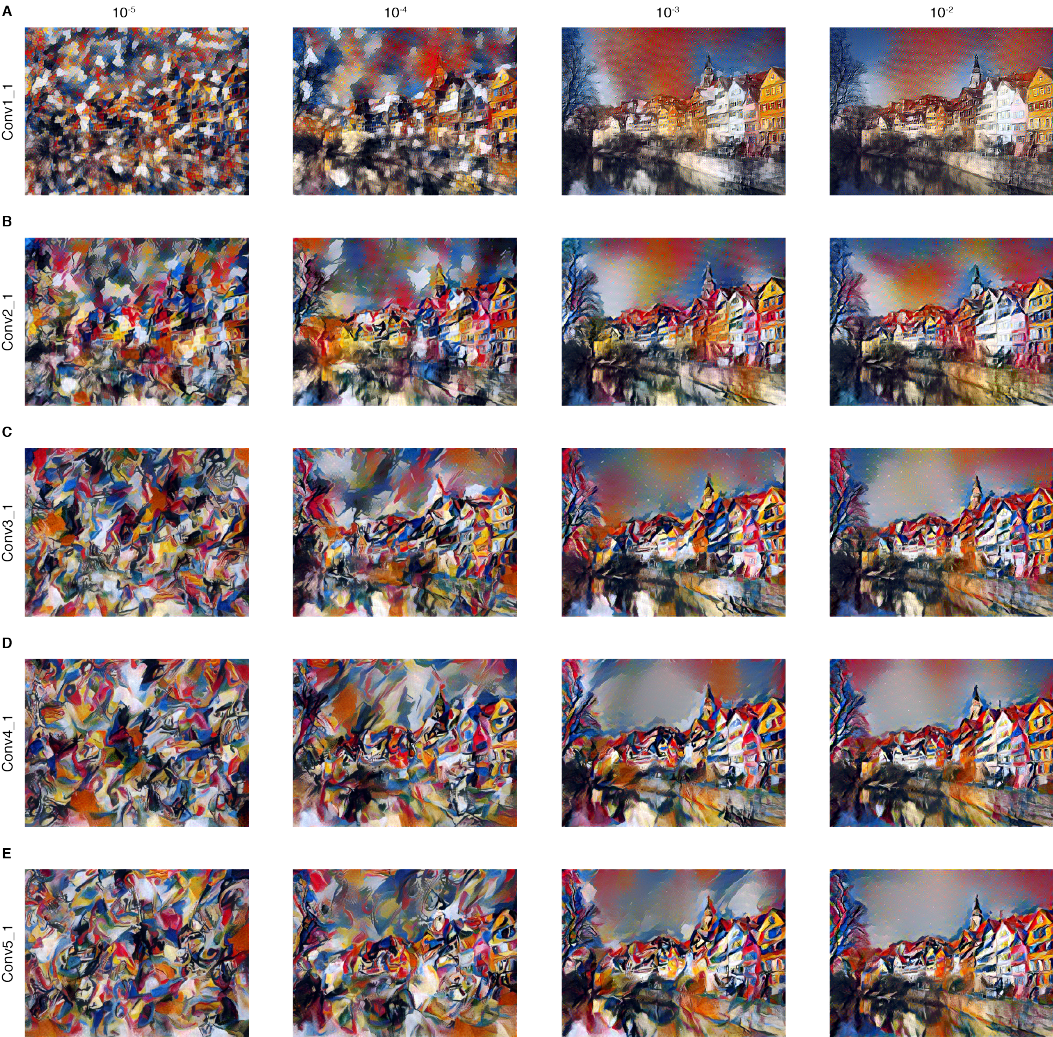
\includegraphics[scale=0.6]{figures/composition.png}
	\caption{Mixing problems}
	\end{figure}
 \end{textblock} 

\end{frame}

\section{Video recognition}

\subsection{Differences in video recognition}
\begin{frame}
\frametitle{Differences in video recognition}
\begin{itemize}

\item First approach: Process each frame individually 
\pause
$\newline$
\item $\rightarrow$ flickering and false continuities 

\end{itemize}

\end{frame}

\begin{frame}

\begin{figure}[h!]
\centering    
\movie[width=1.0\textwidth,height=1.0\textheight,poster
       ,autostart,showcontrols,loop] 
  {
\includegraphics[width=1.0\textwidth]{figures/Black.jpg}}{figures/videoSnippet1.mp4}
  \caption{caption}
 \end{figure} 

\end{frame}




\subsection{Specific problems}
\begin{frame}
\frametitle{Specific Problems}
\begin{itemize}
\item Every frame is initialized with an independent white noise picture 
$\newline$
\pause
$\longrightarrow$ every frame converges differently
$\newline$
\pause
\item Idea: Initialize the optimization for the frame $i + 1$ with the stylized frame $i$
$\newline$
\item Result: Problem with movement of objects

\end{itemize}


\end{frame}

\begin{frame}
\frametitle{Short-term consistency}

\begin{itemize}
\item Estimate optical flow
$\newline$
\item $\longrightarrow$ Warp previous frame: $x'^{(i+1)} = \omega_i^{i+1} (x^{(i)})$

\end{itemize}

\end{frame}

\begin{frame}
\frametitle{Temporal consistency}

\begin{itemize}

\item Stronger consistency between frames needed
$\newline$
\item In some areas we can estimate optical flow with high confidence
$\newline$
\item $\longrightarrow$ extra Loss-function
$\newline$
\item Calculate flow forward and backward $\rightarrow$ should be approximately the same in areas without occlusion

\end{itemize}

\end{frame}

\begin{frame}
\frametitle{Long-term consistency}
Temporally occluded ares should get the same style as before they got occluded.
$\newline \newline \longrightarrow$
Punish deviations from older frames


\end{frame}

\begin{frame}
\frametitle{Multi-pass algorithm}
Problem: low contrast, image boundaries less diverse
$\newline$
$\newline \longrightarrow$ Process sequence multiple times and with different directions


\end{frame}


\subsection{Examples}
\begin{frame}
\begin{figure}[h!]
\centering    
\movie[width=1.0\textwidth,height=1.0\textheight,poster
       ,autostart,showcontrols,loop] 
  {
\includegraphics[width=1.0\textwidth]{figures/Black.jpg}}{figures/video1.mp4}
  \caption{caption}
 \end{figure} 

\end{frame}

\section{Conclusion}
\begin{frame}
\frametitle{Conclusion}

Style transfer in Videos: 
\begin{itemize}
\item suitable initialization
\item shortterm consistency
\item longterm consistency 
\item $\longrightarrow$ Production of stable and stylized videos possible

\end{itemize}
\end{frame}
\section{References}
\begin{frame}
\frametitle{References}
\nocite{*}
\bibliography{lit}
\bibliographystyle{IEEEtran}

\end{frame}





\end{document}